\section{Reglersynthese im Zustandsraum}
\begin{center}
	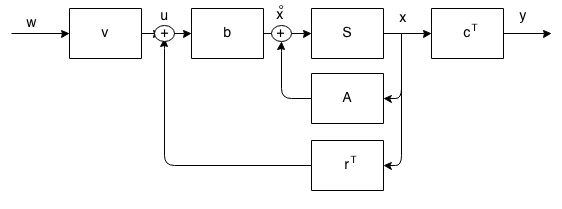
\includegraphics[scale = 0.4]{images/zustandsregler.png}
\end{center}
\[
	A_{CL}= A-b\cdot r^T	\\ A_R=T_R\cdot A \cdot T_R^{-1}
\]
\[
	A_{R,CL}= A_R-b_R\cdot r_R^T	\\	r_R^T=
		\begin{bmatrix}
				r_{1,R}	&	r_{2,R}	& r_{3,R} &r_{n,R}\\
		\end{bmatrix}
\]
Daraus folgt:
\[
		A_{Cl,R}=
		\begin{bmatrix}
			0 &	1 & 0 & .. & 0\\
			0 & 0 & 1 & .. & 0\\
			.. & .. & .. &.. & .. \\
			0 & 0 & 0 & .. & 1\\
				\underbrace{
					-\frac{a_0}{a_n}-r_{1,R} 
				}_{\textbf{$-c^{n-1}$}}
		 &-\frac{a_1}{a_n}-r_{2,R} & -\frac{a_2}{a_n}-r_{3,R} &.. &-\frac{a_{n-1}}{a_n}-r_{n,R}\\	
		\end{bmatrix}
\]
Diese Matrix kann gerade in das Istpolynom überführt werden.
\\
Istpolynom:
\[
	p_{Cl,r}(s)=s^n+
	\underbrace{(a_{n-1}+r_{n,R})	}_{\textbf{$c^{n-1}$}}
	\cdot s^{n-1}+...+(a_{1}+r_{2,R})a_1\cdot s +(a_0+r_{1,r})
\]
Das Sollpolynom ist durch die Nullstellen vorgegeben:
\[
	p(s)=s^n+p_{n-1}\cdot s^{n-1}+...+p_1\cdot s +p_0
\]
Koeffizientenvergleich ergibt nun:
\[
	r_{1,R}=p_0-a_0
\]
\[
	r_{2,R}=p_1-a_1
\]
\[
	r_{n,R}=p_{n-1}-a_{n-1}
\]
\\
\\
Durch die Transformation in RNF der letzten Zeile von $Q_s^{-1}$ (T) lässt sich die Matrix umwandeln.
\[
	r^T=r_R^T \cdot T
\]


\subsection{Vorfilter / Vorverstärker}
Der Vorfilter/Vorverstärker gewährleistet, dass im stationärem Zustand y mit dem gewünschtem, konstantem Vektor w übereinstimmt.
\[
	 	v=[c^T(b\cdot r^T-A)^{-1}\cdot b]^{-1}
\]
\\
\subsection{Beobachter}
Beobachter ist ein Nachbau des System für den Rechner. Er beinhaltet alle Punkte des realen System. Dafür werden keine Sensoren benötigt. Die Variablen werden geschätzt.\\
\\
Das $h$ muss derart bestimmt werden, dass $eigW(A-h_c^T)<0$ sind.\\
\\
Falls das System in BNF vorliegt, gilt:
\[
	A_B=T_B^{-1}\cdot A \cdot T_b	\\	c_B^T=c^T\cdot T_B = [0 \ 0 \ .. \  1]	\\	b_B=T_B^{-1}\cdot b
\]
\[
	A_B= \begin{bmatrix}
				0 &	0 & 0 & .. & -\frac{a_0}{a_n}\\
				1 & 0 & 0 & .. & -\frac{a_1}{a_n}\\
				0 & 1 & 0 & .. & -\frac{a_2}{a_n}\\
				.. & .. & .. &.. & .. \\
				0 & 0 & .. & 1 &-\frac{a_{n-1}}{a_n}\\	
			\end{bmatrix}
\]
Folgende Gleichung wird für die Bestimmung des Istpolynoms benötigt. Da $a_n=1$, kann folgende Vereinfachung gemacht werden:
\[
	\dot{e}_{x,B}=(A_B-h_B\cdot c_B^T)\cdot e_{x,B}=
	\begin{bmatrix}
					0 &	0 & 0 & .. & -a_0-h_{B,1}\\
					1 & 0 & 0 & .. & -a_1-h_{B,2}\\
					0 & 1 & 0 & .. & -a_2-h_{B,3}\\
					.. & .. & .. &.. & .. \\
					0 & 0 & .. & 1 &-a_{n-1}-h_{B,n}\\	
				\end{bmatrix}
\]

Istpolynom:
\[
	u(s)=s^n+(a_{n-1}+h_{B,n})s^{n-1}+...+(a_1+h_{B,2})s+(a_0+h_{B,1})
\]
Sollpolynom:
\[
	p(s)=s^n+p_{n-1}s^{n-1}+...+p_1 s+p_0
\]
Aus diesen beiden Gleichungen kann via Koeffizientenvergleich die Matrix $h_B$ bestimmt werden.
\[
	h_{B,1}=p_0-a_0	\\	h_{B,2}=p1-a1	\\	etc.	
\]
\[
	h_B=p-a
\]